\newcommand{\trigIdentitiesPicture}{
\psset{xunit=1cm,yunit=1cm}
\begin{pspicture}(-4,-0.5)(1,4)
\tiny
\psaxes[labels=none, ticks=none]{<->}(0,0)(-4,-0.5)(1,4)
\fcFullDot{-3}{2}
\psline[linecolor=blue](0,0)(-3,2)
\psline[linecolor=blue](0,0)(1,0)
\psarc[linecolor=red](0,0){0.5}{0}{146.3099}
\rput[br](-3, 2){$(x,y)$}
\rput[l](0.1, 0.7){$\theta$}
\rput[lb](-1.55, 1.1){$r$}
\psline[linestyle=dotted](-3, 2)(-3, 0)
\psline[linestyle=dotted](-3, 2)(0, 2)
\psline(-2.7, 0)(-2.7, 0.3)(-3, 0.3)
\psline(0, 1.7)(-0.3, 1.7)(-0.3, 2)
\end{pspicture}
%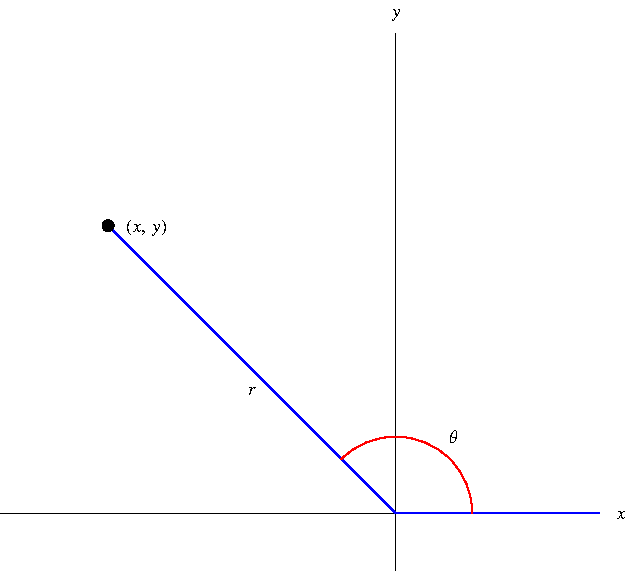
\includegraphics[width=5cm]{trigonometry/pictures/app-d-ratiosb.pdf}%
}

\begin{frame}
\begin{columns}[c]
\column{.45\textwidth}
\trigIdentitiesPicture
\[
\begin{array}{cc}
\sin \theta = \frac{ y}{ r} &
\csc \theta = \frac{ r}{ y} \\
\cos \theta = \frac{ x}{ r} &
\sec \theta = \frac{ r}{ x} \\
\tan \theta = \frac{ y}{ x} &
\cot \theta = \frac{ x}{ y} \\
\end{array}
\]

\vspace{3cm}
\column{.5\textwidth}
\begin{itemize}
\item $\csc \theta = \frac{1}{\sin \theta}$
\item $\sec \theta = \frac{1}{\cos \theta}$
\item $\cot \theta = \frac{1}{\tan \theta}$
\item $\tan \theta = \frac{\sin \theta}{\cos \theta}$
\item $\cot \theta = \frac{\cos \theta}{\sin \theta}$
\end{itemize}
\end{columns}
\end{frame}


\begin{frame}
\begin{columns}[c]
\column{.45\textwidth}
\trigIdentitiesPicture
\[
\begin{array}{cc}
\sin \theta = \frac{ y}{ r} &
\csc \theta = \frac{ r}{ y} \\
\cos \theta = \frac{ x}{ r} &
\sec \theta = \frac{ r}{ x} \\
\tan \theta = \frac{ y}{ x} &
\cot \theta = \frac{ x}{ y} \\
\end{array}
\]

\vspace{3cm}
\column{.5\textwidth}
\begin{eqnarray*}
& & \uncover<2->{\sin^2 \theta + \cos^2 \theta}\\
& \uncover<3->{=} & \uncover<3->{\frac{y^2}{r^2} + \frac{x^2}{r^2}}\\
& \uncover<4->{=} & \uncover<4->{\frac{y^2+x^2}{r^2}}\\
& \uncover<5->{=} & \uncover<5->{\frac{r^2}{r^2}}\\
& \uncover<6->{=} & \uncover<6->{1}
\end{eqnarray*}
\uncover<7->{%
Therefore $\sin^2 \theta + \cos^2 \theta = 1$.%
}%
\end{columns}
\end{frame}

\begin{frame}
\begin{columns}[c]
\column{.45\textwidth}
\trigIdentitiesPicture
\[
\begin{array}{cc}
\sin \theta = \frac{ y}{ r} &
\csc \theta = \frac{ r}{ y} \\
\cos \theta = \frac{ x}{ r} &
\sec \theta = \frac{ r}{ x} \\
\tan \theta = \frac{ y}{ x} &
\cot \theta = \frac{ x}{ y} \\
\end{array}
\]

\vspace{3cm}
\column{.5\textwidth}
\begin{example}[$\tan^2 \theta + 1 = \sec^2 \theta$]
Prove the identity $\tan^2 \theta + 1 = \sec^2 \theta$.
\begin{eqnarray*}
\uncover<2->{\sin^2 \theta + \cos^2 \theta} & \uncover<2->{=} & \uncover<2->{1}\\
\uncover<3->{\frac{\sin^2 \theta}{\cos^2\theta} + \frac{\cos^2 \theta}{\cos^2\theta}} & \uncover<3->{=} & \uncover<3->{\frac{1}{\cos^2\theta}}\\
\uncover<4->{\tan^2 \theta + 1} & \uncover<4->{=} & \uncover<4->{\sec^2\theta}
\end{eqnarray*}
\end{example}
\end{columns}
\end{frame}
